% vim: spelllang=es

\chapter{¿Qué es Tremor?}\label{ch:tremor}

\section{Procesado de Eventos}

Tremor es un \emph{Sistema de Procesado de Eventos}, que consiste en ``el
monitorizado y análisis (procesado) de flujos de información (datos) sobre cosas
que pasan (eventos)''~\cite{luckham2011event}. Tremor fue creado como una
alternativa de alto rendimiento a herramientas como \textcite{logstash} o
\textcite{telegraf}, pero ha evolucionado para soportar casos de uso más
complejos. Al contrario que esos programas, Tremor también tiene soporte para
\emph{agregación} y \emph{rollups}, e incluye un lenguaje \emph{ad hoc} para
\emph{Extract, Transform, and Load} (ETL).

Para más información sobre Tremor se puede consultar \textcite{tremorintro}, que
introduce sus conceptos más básicos y sus posibles usos --- o cuándo \emph{no}
usarlo, en \textcite{tremorconstraints}. \textcite{tremorrecipes} lista un total
de 32 ejemplos de cómo configurar y emplear el software. El
Anexo~\ref{annex:tremor} entra en más detalles sobre su implementación interna.

\textcite{robins2010complex} y \textcite{cugola2012processing} introducen en
detalle los dos campos contenidos en Procesado de Eventos: \emph{Procesado de
Eventos Complejos} y \emph{Procesado de Flujos de
Eventos}\footnote{\emph{Complex Event Processing} y \emph{Event Stream
Processing} respectivamente, siguiendo la terminología anglosajona.}, ambos
relevantes a Tremor. \textcite{dayarathna2018recent} y
\textcite{tawsif2018review} resumen los avances más recientes en el campo,
analizan su evolución, y clasifican sus subáreas. La mayoría de la información
teórica tanto en esta sección como en el Anexo~\ref{annex:tremor} se extrae de
estas fuentes.

\section{Casos de uso}

La Figura~\ref{fig:tremor_example} ilustra uno de los casos de uso más básicos
de Tremor:

\begin{enumerate}
    \item Recibir \emph{logs} (eventos) de aplicaciones en diferentes protocolos
        o formatos. Es posible que esta heterogeneidad se deba a que algunas
        aplicaciones son legadas y no se puedan reducir a un único protocolo o
        formato, o que esta tarea es demasiado compleja como para gestionarse a
        nivel de aplicación.

    \item Filtrar los eventos redundantes, añadir campos nuevos o eliminar
        aquellos innecesarios y transformar todo a un mismo formato. El uso de
        una herramienta ineficiente o \emph{ad hoc} por la empresa podría ser
        inviable dada una cantidad de datos suficientemente grande o demasiados
        protocolos y formatos como para implementarlos todos.

    \item Enviar todos los logs estructurados a una base de datos para
        analizarlos posteriormente.

\end{enumerate}

\begin{figure}
    \centering
    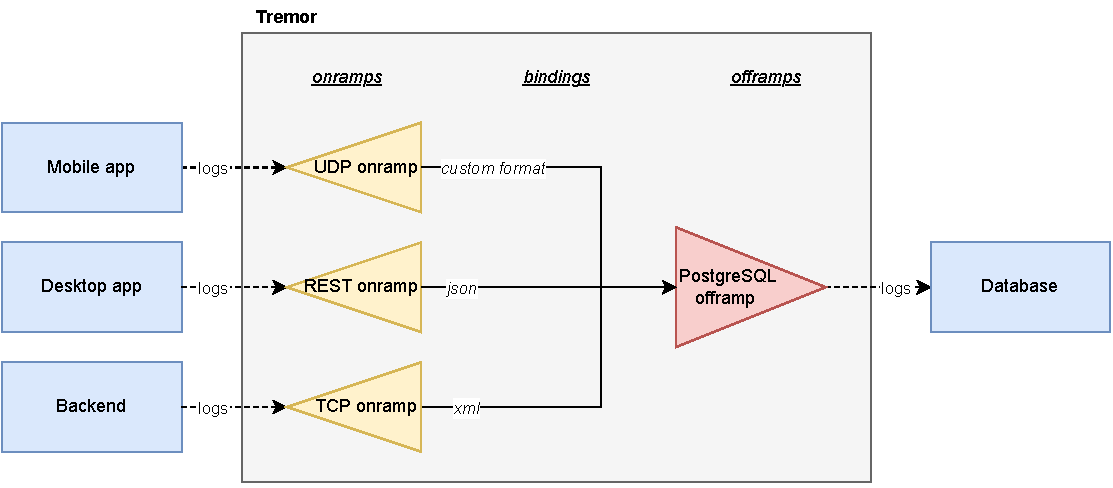
\includegraphics[width=\textwidth]{./Imagenes/example.pdf}
    \caption{Ejemplo de uso básico de Tremor}%
    \label{fig:tremor_example}
\end{figure}

Sin embargo, este caso subestima el potencial de Tremor. La entrada y salida del
sistema se pueden abstraer más, por ejemplo implementando un chatbot que
reproduce música. Este podría tomar mensajes de Discord como su entrada, y
enviar comandos con el API de Spotify como salida.

\section{Conceptos básicos}

Tremor se basa en los términos de \onramps o \sources y \offramps o \sinks:

\begin{itemize}
    \item Una \onramp especifica cómo Tremor se conecta con el mundo exterior (o
        una \pipeline) para \textbf{recibir} de sistemas externos. Por ejemplo
        TCP, periódicamente o PostgreSQL~\cite{tremoronramps}.

    \item Una \offramp especifica cómo Tremor se conecta con el mundo exterior
        (o una \pipeline) para \textbf{enviar} a sistemas externos. Por ejemplo,
        \emph{stdout}, Kafka o ElasticSearch~\cite{tremorofframps}.

    \item Una \pipeline es una lista de operaciones (transformación, agregación,
        eliminación, etc) a través de la cual se pueden encaminar los
        eventos~\cite{tremorpipelines}.

\end{itemize}

Estos \onramps u \offramps suelen contener una cantidad de información que es
demasiado grande como para guardarla y debería tratarse en tiempo real. Su
procesado se basa en las siguientes operaciones:

\begin{itemize}
    \item \emph{Filtros}: descarte de eventos completos a partir de reglas
        configuradas, con el objetivo de eliminar información de la \pipeline
        que no se considera relevante.

    \item \emph{Transformaciones}: conversión de los datos de un formato a otro,
        como por ejemplo incrementar un campo con un contador, reemplazar
        valores, o reorganizar su estructura.

    \item \emph{Matching}: búsqueda de partes de eventos que siguen un patrón en
        específico (por ejemplo, un campo \code{"id"} con un valor númerico)
        para transformarlo o descartarlo.

    \item \emph{Agregación} o \emph{rollups}: recolección de múltiples eventos
        para producir otros nuevos (e.g., la media o máximo de un campo), de
        forma que la información útil se reduzca en tamaño.

\end{itemize}

Finalmente, otros términos misceláneos sobre Tremor:

\begin{itemize}
    \item \emph{Códec}: describen cómo decodificar los datos del flujo y como
        volverlos a codificar. Por ejemplo, si los eventos de entrada usan JSON,
        tendrá que especificarse ese códec para que Tremor lo pueda entender.

    \item \emph{Preprocesador} o \emph{postprocesador}: operadores sobre flujos
        de datos brutos. Un preprocesador aplicará esta operación antes del
        códec y un postprocesador después. Por ejemplo, \code{base64} codifica o
        decodifica la información con ese protocolo.

    \item \emph{Artefacto}: término genérico para hablar de \sinks, \sources,
        códecs, preprocesadores y postprocesadores.

\end{itemize}

\section{Conectores}

Es posible que algunas \onramps no solo quieran recibir de sistemas externos,
sino también responderles directamente, actuando como una \offramp y viceversa.
Esto es especialmente útil para casos como REST y \websockets, donde el
protocolo da la posibilidad de responder a eventos, por ejemplo con un ACK,
usando la misma conexión. En la versión 0.11 --- la presente cuando me uní al
proyecto --- este problema se solucionaba con el concepto de \emph{linked
transports}.

El término \emph{conector} se introdujo en mayo de 2022 con la versión 0.12.
Solucionan el problema desde el inicio, abstrayendo tanto los \onramps como los
\offramps bajo el mismo concepto, incluyendo los \emph{linked transports}. Dado
que estos ya estaban siendo desarrollados mientras 0.11 era la última versión,
el sistema de plugins se enfocó a los conectores desde el principio, en lugar de
\onramps u \offramps, que ahora han quedado en desuso.
